


\documentclass{article}[12pt]
\usepackage{fullpage,graphicx, setspace, latexsym, cite,amsmath,amssymb,color}
%\usepackage{epstopdf}
%\DeclareGraphicsExtensions{.pdf,.eps,.png,.jpg,.mps} 
\usepackage{amssymb} %maths
\usepackage{amsmath} %maths
\usepackage{amsthm}
\usepackage{mathtools}
\usepackage[draft]{commands}
\usepackage[parfill]{parskip}
\usepackage{listings}
\usepackage{mcode}
%\usepackage{caption}
\usepackage{subcaption}

\bibliographystyle{unsrt}

%\newtheorem{theorem}{Theorem}
\newtheorem{prop}{Proposition}
\newtheorem{corollary}{Corollary}
%\newtheorem{lemma}{Lemma}
\newtheorem{defn}{Definition}
\newtheorem{ex}{Example}
\usepackage{float}

%\def\R{\mathbb{R}}
%\def\Eps{\mathcal{E}}
%\def\E{\mathbb{E}}
%\def\V{\mathbb{V}}
%\def\F{\mathcal{F}}
%\def\G{\mathcal{G}}
%\def\H{\mathcal{H}}
%\def\S{\mathcal{S}}
%\def\P{\mathbb{P}}
%\def\1{\mathbf{1}}
%\def\n{\nappa}
%\def\h{\mathbf{w}}
%\def\v{\mathbf{v}}
%\def\x{\mathbf{x}}
%\def\X{\mathcal{X}}
%\def\Y{\mathcal{Y}}
%\def\eps{\epsilon}
%\def\y{\mathbf{y}}
%\def\e{\mathbf{e}}
%\newcommand{\norm}[1]{\left|\left|#1\right|\right|}
%\DeclareMathOperator*{\argmin}{arg\,min}
%\DeclareMathOperator*{\argmax}{arg\,max}

\newcommand{\lecture}[4]{
   \pagestyle{myheadings}
   \thispagestyle{plain}
   \newpage
   % \setcounter{lecnum}{#1}
   \setcounter{page}{1}
   \setlength{\headsep}{10mm}
   \noindent
   \begin{center}
   \framebox{
      \vbox{\vspace{2mm}
    \hbox to 6.28in { {\bf ESE 680-004: Learning and Control
   \hfill Fall 2019} }
       \vspace{4mm}
       \hbox to 6.28in { {\Large \hfill Lecture #1: #2  \hfill} }
       \vspace{2mm}
       \hbox to 6.28in { {\it Lecturer: #3 \hfill Scribes: #4} }
      \vspace{2mm}}
   }
   \end{center}
   \markboth{Lecture #1: #2}{Lecture #1: #2}

   \noindent{\bf Disclaimer}: {\it These notes have not been subjected to the
   usual scrutiny reserved for formal publications. }
   \vspace*{4mm}
}

%notation
\def \E{\mathbb E}
\def \P{\mathbb P}
\def \R{\mathbb R}
\def \A{\cal A}


\begin{document}

\lecture{4}{Finite-data guarantees and data-dependent bounds}{Nikolai Matni}{Kuk Jang}

\section{Recap}

Recall that we were analyzing the scalar dynamical system
\begin{align*}
x_{t+1} = ax_t + u_t + w_t \\ 
x_0 = 0
\end{align*}
where $w_{t} \iid \Ncal(0, \sigma_w^2)$, $u_{t} \iid \Ncal(0, \sigma_u^2) $,
and $a$, $x$, $u$, $w \in \R$. 

We ran $N$ experiments and then solved for the estimate $\hat{a}$ via least-squares 

\begin{align*}
\hat{a} &= \arg \min_a \sum_{i=1}^{N} (x_{T+1}^{(i)} - ax_{T}^{(i)} - u x_{T}^{(i)})^2 \\
&= a + \frac{|\sum_{i=1}^{N} x_T^{(i)} w_T^{(i)}| }{\sum_{i=1}^{N} (x_T^{(i)})^2} \\
&\coloneqq a + e_N 
\end{align*}
To analyze $e_N$, where,  

\begin{align}
|e_N| = \frac{|\sum_{i=1}^{N} x_T^{(i)} w_T^{(i)}| }{\sum_{i=1}^{N} (x_T^{(i)})^2}
\end{align}

We divide the problem into two problems:
\begin{enumerate}
	\item Find a high probability upper bound on numerator
	\item Find a high probability lower bound on denominator
\end{enumerate} 

\section{Lower bound on denominator, $\sum_{i=1}^{N} (x_T^{(i)})^2$}
Deriving the bounds requires us to assume that we utilize only the last two data-points from each trial in order to simplify the analysis. 

How to utilize all the data (the single trajectory case) and derive high probability bounds is presented in a subsequent lecture. 

\begin{prop}
	\label{prop:lb}
	Fix a failure probability $\delta \in (0, 1]$, and let $ N \geq 32\log(\frac{1}{\delta})$.
	Then with probability at least $1-\delta$, we have that
	\begin{align}
	\sum_{i=1}^{N} (x_T^{(i)})^2 \geq \sigma_x^2 \frac{N}{2}
	\end{align}
	where, $\sigma_x^2 \coloneqq (\sigma_w^2 + \sigma_u^2) + \sum_{t=0 }^{T-1} a^{2t}$
\end{prop}

\begin{proof}
	%\emph{Note, in general the approach for these types of proofs is to start with some basic random variable for which you know how to integrate and can solve for closed form and then utilize the properties to extract the behavior of our target.}
	
	From previous examples, we know that for $X\sim \Ncal(0,1)$, $X^2$ is sub-exponential with parameters (4,4). 
	We saw that if $X_1$ and $X_2$ are sub-exponential with parameters $(\nu^2_i, \alpha_i)_{i=1,2}$, then $X_1 +X_2$ is sub-exponential with parameters $(\nu_1^2 + \nu_2^2, \max{\alpha_1, \alpha2})$. 
	
	We let $\sigma_x^2 = \E x^2_T$ (the variance of our state).
	Since $X_T$ is Gaussian, dividing by it's standard deviation yields a standard normal distribution, 
	$
	\frac{x_T}{\sigma_T} \sim \Ncal(O,1)
	$.
	
	From this, we know that
	$\frac{x^2_T}{\sigma^2_T}$ is sub-exponential(4,4) with mean 1 and 
	$\sum_{i=1}^{N}\frac{(x^2_T)^(i)}{\sigma^2_x}$ is sub-exponential (4N,4) with mean N.
	
	We apply $\P[X-\E X \geq t] \leq \exp{\frac{-t^2}{2\nu^2}}$  if $0 \leq t \leq \nu^2/\alpha$ to $\sum_{i=1}^{N}\frac{(x^2_T)^{(i)}}{\sigma^2_x}$ and derive the bounds with respect to $N$. 
	
	\begin{align*}
	\P \left[ \sum x_T^{(i)^2} - N \sigma_x^2 \leq -t\right]
	&= \P \left[\sigma_x^2 \left[\sum\frac{(x_T^{(i)})^2}{\sigma_x^2} - N\right] \leq t\right] \\
	&= \P \left[\sum\frac{(x_T^{(i)})^2}{\sigma_x^2} - N \leq \frac{-t}{\sigma_x^2} \right] \leq \exp{\frac{-t}{8N\sigma_x^4}} & \forall t \leq N\sigma_x^2
	\end{align*}
	
	We invert this expression by setting $\delta = RHS$, and solving for $t$
	
	\begin{align*}
	t &= \sigma_x^2 \sqrt{8N\log(1/\delta)} \leq N\sigma_x^2 &\text{(assumed $N \geq 32 \log(1/\delta)$)}
	\end{align*}
	
	So we've shown that:
	\begin{align*}
	\sum \left(x_T^{(i)}\right)^2 \geq \underbrace{N\sigma_x^2}_{\E \sum x_T^2} - \underbrace{\sigma_x\sqrt{8N\log(1/\delta)}	}_{\text{error term}}
	\end{align*}
	Since
	\begin{align*}
	N \geq 32\log(1/\delta) \geq \sigma_x^2 \frac{N}{2}
	\end{align*}
\end{proof}

	Comments:
	Why is $
	\frac{x_T}{\sigma_T} \sim \Ncal(O,1)
	$? Nice things happen when linear systems are driven by Gaussian noise.
	\begin{enumerate}
		\item 
		
		If,
		$x_{t+1} = ax_t + u_t + w_t$, 
		$x_0 = 0$, 
		$w_{t} \iid \Ncal(0, \sigma_w^2)$, 
		$u_{t} \iid \Ncal(0, \sigma_u^2) $, 
		
		we first compute the first moment, 
		\begin{align*}
		X_1 &= AX_0 + B u_0 + w_0 = Bu_0 + w_0 \\
		\E[X_1] &= \E(B u_0 + w_0 ) = B \E[u_0] + E[w_0]  = 0 &\\
		\end{align*}
		 
		
		\item We compute the second moment $\sigma_x^2 = \E[X_T^2]$ using induction.
		\begin{align*}
		X_{T} &= aX_{T-1} + u_{T-1} + w_{T-1} \\
		X_{T-1} &= aX_{T-2} + u_{T-2} + w_{T-2} \\
		&\vdots \\
		X_{1} &= aX_{0} + u_{1} + w_{1}\\
		\downarrow \\
		X_T &= a^Tx_0 + \sum_{t=0}^{T-1} a^{t-1}(u_{T-t}+ w_{T-t})
		\end{align*}
		Expanding terms and using linearity of expectation we obtain, 
		\begin{align*}
		\E[X_T^2] &= \E[(\sum_{t=0}^{T-1} a^{t-1}(u_{T-t}+ w_{T-t})) \cdot (\sum_{t=0}^{T-1} a^{t-1}(u_{T-t}+ w_{T-t}))]
		\end{align*}.
		Since $w_{t} \iid \Ncal(0, \sigma_w^2)$, $u_{t} \iid \Ncal(0, \sigma_u^2) $,
		\begin{align*}
		\E[w_t w_\tau] &= \begin{cases}
		0 & \text{ if $t \neq \tau$}\\
		1 & \text{ if $t = \tau$}
		\end{cases}\\
		\E[u_t w_\tau] & = 0 & \text{ $\forall t, \tau$}
		\end{align*}
		Therefore,
		\begin{align*}
		\E[X_T^2] &= \sum_{t=0}^{T-1}a^{t-2}(\underbrace{\E[u_t^2]}_{\normalfont \sigma_u^2} + 
		\underbrace{\E[w_t^2]}_{\normalfont \sigma_w^2})
		\end{align*}
		
		%\item (s.18) Also holds for general random variables.
		
	\end{enumerate}


\section{Upper bound on numerator, $|\sum_{i=1}^{N} x_T^{(i)} w_T^{(i)}| $}

In order to find the upper bound we first state the following proposition;
\begin{prop}
	\label{prop:ub}
	Fix a failure probability $\delta \in (0, 1]$, and let $ N \geq 2\log(\frac{1}{\delta})$.
	Then with probability at least $1-\delta$, we have that
	\begin{align}
	\lVert \sum_{i=1}^{N} x_T^{(i)}w_T^{(i)}  \rVert \leq 2\sigma_x\sigma_w \sqrt{N\log(2/\delta)} 
	\end{align}
	where, $\sigma_x^2 \coloneqq (\sigma_w^2 + \sigma_u^2) + \sum_{t=0 }^{T-1} a^{2t}$
\end{prop}

Before we go into the proof, observe the following:
\begin{itemize}
	\item In the previous section, we showed that the denominator $\succsim N$. 
	From the proposition, the numerator  $\precsim \sqrt{N}$. 
	Therefore, $e_N \precsim \frac{1}{\sqrt{N}}$. 
	\item This relates to a tradeoff between how many trials vs. how long I can run each trial. %If my system is stable, limits to how long I can run. If my system is unstable \ldots
	%\item Barely unstable $\leftarrow$ may be identified as stable.
\end{itemize}
\begin{proof}
	\emph{(sketch)}
	From previous examples, we know that for $X,W \iid \Ncal(0,1)$, $XW$ is sub-exponential with parameters $(2,\sqrt{2})$. 
	We saw that if $X_1$ and $X_2$ are sub-exponential with parameters $(\nu^2_i, \alpha_i)_{i=1,2}$, then $X_1 +X_2$ is sub-exponential with parameters $(\nu_1^2 + \nu_2^2, \max{\alpha_1, \alpha2})$. 
	
	Letting $\sigma_x^2 = \E x^2_T$,
	$
	\frac{x_T}{\sigma_T} \text{ and } \frac{w_T}{\sigma_T} \iid \Ncal(O,1)
	$.
	
	From this, we know that
	$\frac{x_T}{\sigma_T}\frac{w_T}{\sigma_T}$ is sub-exponential$(2,\sqrt{2})$ and 
	$\sum_{i=1}^{N}\frac{(x_T)^{(i)}(w_T)^{(i)}}{\sigma_x\sigma_w}$ is sub-exponential $(2N,\sqrt{2})$ with mean N.
	
	We apply $\P[X-\E X \geq t] \leq \exp(\frac{-t^2}{2\nu^2})$  if $0 \leq t \leq \nu^2/\alpha$ to $\sum_{i=1}^{N}\frac{(x_T)^(i)(w_T)^(i)}{\sigma_x\sigma_w}$ similar to before.
	
\end{proof}

From Proposition \ref{prop:lb} and Proposition \ref{prop:ub}, we obtain the following theorem:

\begin{theorem}
	Fix a failure probability $\delta \in (0,1]$ and let $N \geq 32 \log(\frac{2}{\delta})$. Then with probability $1-\delta$, 
	\begin{align*}
	\lvert e_N \rvert = \frac{\lvert \sum_{i=1}^{N} x_t^{(i)}w_t^{(i)}\rvert}{\sum_{i=1}^{N}(x_T^{(i)})^2}
	\leq 4 \frac{\sigma_w}{\sigma_x} \sqrt{\frac{\log(2/\delta)}{N}}
	\end{align*}
\end{theorem}

\begin{proof}
	The proof is based on the choice of N where we can show that the numerator is big with probability $\leq \delta/2$ and that the denominator is small with probability $\leq \delta/2$, then union bound.
\end{proof}
\section{Full state system ID with IID trials}

\subsection{Overview}
Let us now examine the full state linear time invariant system:
\begin{align*}
x_{t+1} = Ax_t + Bu_t + w_t
\end{align*} 
 
with $w_{t} \iid \Ncal(0, \sigma_w^2 I_n)$, 
$x \in \R^n$,
control input
$u_{t} \in \R^p$,
disturbance
$w \in \R^n$

Our goal is to identify the unknown $(A,B)$. 
To do this, we run $N$ experiments over a horizon of $T+1$ steps, injecting random inputs $u_t \iid \Ncal(0, \sigma^2_u I_p)$ to generate the set $\{x^(i)_{0:T+1}, u^(i)_{0:T+1}\}_{i=1}^N$.

We solve the OLS: $(\hat{A}, \hat{B}) = \arg\min_{(A,B)}\sum_{i=1}^{N} \norm{x_{T+1}^{(i)} - Ax_{T}^{(i)}- Bu_{T}^{(i)}}$.
Notice, we are only summing the last two data points so that the terms in the sum are i.i.d.\

We wish to characterize the convergence rate properties of the estimates:
$(\hat{A}, \hat{B}) \rightarrow(A,B)$.

\subsection{Notation}
In order to simplify the arguments following, we first define some notation:

Let
\begin{align*}
X_N \coloneqq 
\begin{bmatrix}
(x_{T+1}^{(1)})^\top\\
\vdots\\
(x_{T+1}^{(N)})^\top
\end{bmatrix},
Z_N \coloneqq 
\begin{bmatrix}
(x_{T+1}^{(1)})^\top, (u_{T+1}^{(1)})^\top\\
\vdots\\
(x_{T+1}^{(N)})^\top,(u_{T+1}^{(N)})^\top
\end{bmatrix},
W_N \coloneqq 
\begin{bmatrix}
(w_{T+1}^{(1)})^\top\\
\vdots\\
(w_{T+1}^{(N)})^\top
\end{bmatrix}
\end{align*}
Then we can rewrite
\begin{align*}
\begin{bmatrix}
\hat{A} & \hat{B}
\end{bmatrix}^\top
&=\arg\min_{(A,B)}\sum_{i=1}^{N} \norm{x_{T+1}^{(i)} - Ax_{T}^{(i)}- Bu_{T}^{(i)}}\\
&= \arg \min_{(A,B)} \norm{X_N - Z_N [A \quad B]^\top} ^2_F \\
&= [A \quad B]^\top + (Z_N^\top Z_N)^{-1}Z_N^\top W_N
\end{align*} 
where, 
\begin{align*}
Z_N^\top W_N & = \sum_{i=1}^{N} \begin{bmatrix}
x_T^{(i)} \\ u_T^{(i)}
\end{bmatrix}
(w_T^{(i)})^\top \\
Z_N^\top Z_N & = \sum_{i=1}^{N} 
\begin{bmatrix}
x_T^{(i)} \\ u_T^{(i)}
\end{bmatrix}
\begin{bmatrix}
x_T^{(i)} \\ u_T^{(i)}
\end{bmatrix}^\top
\end{align*}

Notice that $Z_N^\top Z_N $ acts as the \emph{denominator} and $Z_N^\top W_N$ acts as the \emph{numerator}.  

From this, we can define the error in $(A,B)$, i.e., spectral norm bounds, as
\begin{align*}
E_A \coloneqq (\hat{A}-A)^\top &= 
\begin{bmatrix}
I_{n_x} & 0_{n_x \times n_u}
\end{bmatrix}
(Z_N^\top Z_N)^{-1}Z_N^\top W_N \\
E_B \coloneqq (\hat{B}-B)^\top &= 
\begin{bmatrix}
0_{n_x \times n_u} & I_{n_u}
\end{bmatrix}
(Z_N^\top Z_N)^{-1}Z_N^\top W_N 
\end{align*}.

\subsection{Error bounds for $E_A$ and $E_B$}
We will focus on $E_A$.  Similar arguments hold for $E_B$.

We know that $w_t \iid \Ncal(0, \sigma_w^2I_n)$.

For,
$\begin{bmatrix}
x_T^{(i)} & u_T^{(i)}
\end{bmatrix}^\top$,

Through an inductive argument, we can derive that 
\begin{align*}
X_T = \sum_{t=1}^{T}A^{t-1}(Bu_{T-t-1}+w_{T-t-1})
\end{align*}
By the linearity of expectation
\begin{align*}
\E X_T = 0
\end{align*}
similarly, 
\begin{align*}
\E X_T X_T^\top = \sum_{t=1}^{T} A^{t-1}BB^\top (A^{t-1})^\top \sigma_u^2 
+ \sum_{t=1}^{T} A^{t-1}(A^{t-1})^\top \sigma_w^2
\end{align*}

Therefore, 
\begin{align*}
\begin{bmatrix}
x_T^{(i)} \\
u_T^{(i)}
\end{bmatrix}
\iid
\Ncal\left(0, 
\begin{bmatrix}
\sigma_u^2 \Lambda_C(A,B,T) + \sigma_w^2 \Lambda_C(A,I,T) & 0 \\
0 & \sigma_u^2 I_{n_u}
\end{bmatrix}
\right)
\end{align*}
where, $\Lambda_C(A,B,T) = \sum_{t=0}^{T} A^t BB^\top (A^\top)^t$ is the $T$-step controllability Grammian.
Note that the singular values of the grammian relates to how easy the system is to identify.

Now we derive the bounds on $\norm{\hat{A} - A } _2$,
Define $Q_A = [I_{n_x} \, 0_{n_x \times n_u}]$, then 

\begin{align*}
\norm{\hat{A} - A } & = 
\norm{Q_A (Z_N^\top Z_N)^{-1}Z_N^\top W_N} \\
& = \norm{Q_A (\Sigma_x^{1/2}Y_N^\top \Sigma_x^{1/2})^{-1}\Sigma_x^{1/2}Y_N^\top W_N} \\
& = \norm{Q_A \Sigma_x^{-1/2}(Y_N^\top Y_N)^{-1}Y_N^\top W_N}\\
& = \norm{[\Sigma_x^{-1/2} \quad 0](Y_N^\top Y_N)^{-1}Y_N^\top W_N}
\intertext{(via the sub-multiplicative property of the spectral norm)}
&\leq \norm{\Sigma_x^{-1/2}} \frac{\norm{Y_N^\top W_N}}{\lambda_{min}(Y_N^\top Y_N)}
= \lambda_{min}^{-1/2}(\Sigma_x) \frac{\norm{Y_N^\top W_N}}{\lambda_{min}(Y_N^\top Y_N)}
\end{align*}
where $Y_N \coloneqq [y_{i}^\top]_{i=1}^N$, with $y_i \iid \Ncal(0, I_{n_x+n_u})$

In a similar manner, it can be shown that
\begin{align*}
\norm{\hat{B}-B}_w \leq \frac{1}{\sigma_u}
\frac{\norm{Y_N^\top W_N}_2}{\lambda_{min}(Y_N^\top Y_N)}
\end{align*}

\section{Proof Strategy}
In order to derive the bounds, similar to the scalar case:
%\emph{TODO: need to write connection text}
\begin{itemize}
	\item First, find high probability upper bound on $\norm{Y_N^\top W_N}_2$
	\item Next, find high probability lower bound on $\lambda_{min}(Y_N^\top Y_N)$
	\item Union bound to combine the two bounds, similar to before. 
	\item Need only one other trick to use scalar random variable concentration bounds to control the singular values of random matrices
	\item Start with upper bound
	\item Use the variational form of operator norm, pointwise bound, plus a covering argument
\end{itemize} 

\section{Upper bound on $\norm{Y_N^\top W_N}_2$}
First, we state the result, 

\begin{prop}
	\label{prop:ub2}
Let $x_i \in \R^n$ and $w_i \in \R^m$ be such that $x_i \iid \Ncal(0, \Sigma_x)$ and $w_i \iid N(0, \Sigma_w)$, and let $M = \sum_{i=1}^{N} x_i w_i^\top$. Fixing a failure probability $\delta \in (0,1]$ and let $N \geq \frac{1}{2} (n+ m)\log(9/\delta)$. Then, with probability at least $1-\delta$
\begin{align*}
\norm{M} \leq 4 \norm{\Sigma_x}^{1/2}\norm{\Sigma_w}^{1/2}
\sqrt{N(n+m)\log(9/\delta)}
\end{align*}
\end{prop}
Note how the bound depends on $n+m$, meaning it depends on the size of the system.  

\begin{proof}
	Define 
	\begin{align*}
	M &= \Sigma_x^{1/2} (\Sigma_{i=1}^N Y_i Z_i^T) \Sigma_w^{1/2} & \text{where $Y_i \sim N(0, I_n), Z_i \sim N(0, I_m)$}\\
	\norm{M} & \leq \norm{\Sigma_x^{1/2}}\norm{\Sigma_w^{1/2}} \norm{\Sigma_{i=1}^N Y_i Z_i^T) }
	\end{align*}
	Here,
	\begin{align*}
	\norm{\Sigma_{i=1}^N Y_i Z_i^T) }_2 &= \sup \sum_{i=1}^{N} (u^\top y_i)(z_i^\top v) & \text{where $\norm{u}=\norm{v} =1$, $u\in \R^n$, $v \in \R^m$}
	\end{align*}
	
	It's at this point that we approximate the supremum with an $\epsilon$-net. 
	
	\begin{definition}[$\epsilon$-net]
		(HDP, Ch. 4.2)
		Let $(T,d)$ be a metric space. Consider a subset $K \subset T$ and let $\epsilon>0$.
		A subset $\Ncal \subseteq K$ is called an \emph{$\epsilon$-net of $K$} if every point in $K$ is within distance $\epsilon$ of some point $\Ncal$, i.e.
		\begin{align*}
		\forall x \in K \exists x_0 \in \Ncal : d(x, x_0)\leq \epsilon
		\end{align*}
 	\end{definition}
 Equivalently, $\Ncal$ is an $\epsilon$-net of $K$ if and only if $K$ can be covered by balls with centers in $N$ and radii $\epsilon$. 
 
 \begin{definition}[Covering numbers]
 	The smallest possible cardinality of an $\epsilon$-net of $K$ is called the \emph{covering number} of $K$ and is denoted $\Ncal (K, d, \epsilon)$. Equivalently, $\Ncal (K, d, \epsilon)$ is the smallest number of closed balls with centers in $K$ and radii $\epsilon$ whose union covers $K$.
 \end{definition}
	
	
	Using the $\epsilon$-net trick which grids up the space, 
	
	Let $\{u_k\}_{k=1}^{N_\epsilon}, \{v_k\}_{k=1}^{M_\epsilon}$ be such that,
	\begin{align*}
	\forall \norm{u} =1, \norm{u- u_k} &\leq \epsilon & \text {for some $u_k$}\\
	\forall \norm{v} =1, \norm{v- v_k} &\leq \epsilon & \text {for some $v_k$}
	\end{align*} 
	In other words they are the $\epsilon$-coverings of the $\mathcal{S}^{n-1}$ and $\mathcal{S}^{m-1}$, respectively. 
	Then,
	\begin{align*}
	u^\top M v &= (u-u_k^\top)Mv + u_k^\top M(v-v_l) + u_k^\top Mv_l \\
	&\leq \norm{u-u_k}\norm{M}\norm{v} + \norm{u_k}\norm{M}\norm{v-v_l} + u_k^\top Mv_l \\
	& = 2\epsilon\norm{M} + \max_{k,l} u_k^\top Mv_l
	\end{align*} 
	Taking the supremum, 
	\begin{align*}
	\norm{M} &\leq 2\epsilon \norm{M} + \max_{k,l} u_k^\top Mv_l\\
	\norm{M} &\leq \frac{1}{1-2\epsilon}\max_{k,l} u_k^\top Mv_l
	\end{align*}
	If we set $\epsilon= 1/4$ and do a standard volume comparison, then we can show that
	\begin{align*}
	N_\epsilon &\leq 9^m \\
	M_\epsilon &\leq 9^n
	\end{align*}
	So the total number of pairs $(u_k, v_k) \leq 9^{n+m}$  
	Substituting back in, we get 
	\begin{align*}
	\norm{\Sigma_{i=1}^N Y_i Z_i^T) }_2 &\leq 2 \max_{1 \leq k \leq 9^n, 1\leq l \leq 9^m} \sum_{i=1}^{N} (w_k^\top y_i )(z_i^\top v_l) \\
	\norm{\Sigma_{i=1}^N Y_i Z_i^T) }_2 &\leq 2 \sum_{i=1}^{N} (u_k^\top y_i)(z_i^\top v_l) & \text{$\forall 9^{(m+n)}$ $(u_k,v_l)$ pairs}
	\end{align*}
	
	Applying the sum of sub-exponential r.v.s concentration bounds with probability of failure $\frac{\delta}{9^{n+m}}$. Then with probability $1- \frac{\delta}{9^{n+m}}$
	\begin{align*}
	\sum(u_k^\top y_i )(z_t^\top v_l ) \leq 2 \sqrt{N\log(\frac{9^{n+m}}{\delta})} \leq 2\sqrt{N(n+m) \log \frac{1}{\delta}}
	\end{align*}
	Union bound over all $9^{n+m}$ such events to get the result. 
	Additional details can be found in \cite{matni_tutorial_2019}
\end{proof}
\section{Lower bound on $\lambda_{min}(Y_N^\top Y_N)$}
Using a similar approach, we obtain the lower bound.
\begin{prop}
	\label{prop:lb2}
	Let $x_i \in \R^n$ be drawn i.i.d.\ from $\Ncal(0, \Sigma_x)$, and set $M = \sum_{i=1}^{N} x_i x_i^\top$. Fix a failure probability $\delta\in (0, 1]$ and let $N \geq 24n \log(9/\delta)$. Then with probability at least $1-2\delta$, 
	\begin{align*}
	\lambda_{min}(M) \geq \lambda_{min}(\Sigma_x)N/2
	\end{align*}
\end{prop}

\begin{proof}
	The proof utilizes the previous results and an additional covering argument. 
	Refer to \cite{matni_tutorial_2019}
\end{proof}
\section{Putting it all together}
With Proposition \ref{prop:ub2} and Proposition \ref{prop:lb2}, we union bound over all of the relevant failure probabilities. 

\begin{theorem}
	Fix a failure probability $\delta \in (0, 1]$ and assume that $N \geq 24(n_x + n_u) \log(54/\delta)$. 
	Then it holds that with probability at least $1-\delta$, 
	\begin{align*}
	\norm{\hat{A}-A}_2 &\leq 8\sigma_w \lambda_{min}^{-1/2}(\Sigma_x) \sqrt{\frac{(2n_x+n_u)\log(54/\delta)}{N}} \\
	\norm{\hat{B}-B}_2 &\leq 8\frac{\sigma_w}{\sigma_u}  \sqrt{\frac{(2n_x+n_u)\log(54/\delta)}{N}}
	\end{align*} 
\end{theorem}

Note, different bounds with better constants can be found in \cite{dean_sample_2017}.

\section{Data dependent bounds}
The previous results rely on properties of the true underlying system and therefore cannot be used to implemented in practice. 
Therefore, two data-dependent approaches are used to compute error estimates.

\begin{proposition}
Assuming we have $N$ idependent samples ($y^{(l)}, x^{(l)}, u^{(l)})$ such that
\begin{align*}
y^{(l)} =  Ax^{(l)}+ Bu^{(l)} + w^{(l)}),
\end{align*}
where $w^{(l)} \iid \Ncal(0, \sigma^2_w I_{n_x}) $ and are independent from $x^{(l)}$ and $u^{(l)}$. Assume that $N \geq n_x + n_u$, Then with probability $1-\delta$, we have 
\begin{align*}
\begin{bmatrix}
(\hat{A}-A)^\top \\
(\hat{B}-B)^\top
\end{bmatrix}
\begin{bmatrix}
(\hat{A}-A)^\top \\
(\hat{B}-B)^\top
\end{bmatrix}^\top
\preceq C^2_{n_x, n_u, \delta} 
\left( \sum_{l=1}^{N} 
\begin{bmatrix}
x^{(l)}\\
u^{(l)}
\end{bmatrix}
\begin{bmatrix}
x^{(l)}\\
u^{(l)}
\end{bmatrix}^\top
\right)^{-1}
\end{align*}, 
where $C^2_{n_x, n_u, \delta} = \delta^2_w(\sqrt{n_x+n_u}+\sqrt{n_x }+ \sqrt{2\log(1/\delta)})^2$.
If the right hand side has zero as an eigenvalue, we define the inverse of that eigenvalue to be infinity. 
\end{proposition}
The proof can be found in \cite{dean_sample_2017}.

We can obtain better bounds by utilizing the bootstrap technique \cite{efron_bootstrap_1979}. Lecture notes regarding bootstrap can be found in \cite{cmu_lect_13}.
The algorithm can be found in \cite{matni_tutorial_2019}.

\section{Numerical example}
In order to demonstrate the previous results, we apply these methods to estimating the parameters in a planar model for a quadrotor. 

%\begin{figure}[tb]
%	\centering
%	\includegraphics[width=0.3\textwidth]{drone-clipart-8.png}
%	\caption{\small We apply the results to a planar quadrotor model linearized around the hover state.}
%	\label{fig:architecture}
%\end{figure}

More complicated formulations of the dynamics of a quadrotor are possible, but we linearize the dynamics around the hover state for a quadrotor.
The resulting state-space model can be expressed as follows (Assuming full observability):
\begin{align*}
\mathbf{x}_{k+1} = A\mathbf{x}_{k} +B\mathbf{u}_{k}
\end{align*}
where,
\begin{align*}
\mathbf{x} = 
\begin{bmatrix}
x \\
y \\
z \\
\dot{x}\\
\dot{y}\\
\dot{z}\\
\end{bmatrix},
\mathbf{u} = 
\begin{bmatrix}
r \\
p \\
t \\
\end{bmatrix}
A_k = 
\begin{bmatrix}
1 & 0 & 0 & 0.1 &0 &0\\
0 & 1 & 0 & 0 &0.1 &0\\
0 & 0 & 1 & 0 &0 &0.1\\
0 & 0 & 0 & 1 &0 &1\\ 
0 & 0 & 0 & 0 &1 &1\\ 
0 & 0 & 0 & 0 &0 &1\\  
\end{bmatrix}
\,
B_k = 
\begin{bmatrix}
0.049 & 0 & 0 \\
0 & 0.049 & 0 \\
0 & 0 & 0.01 \\
0.98 & 0 & 0 \\
0 & -0.98 & 0 \\
0 & 0 & 0.2 \\
\end{bmatrix}
\end{align*}
We set the parameters, gravity $g = 9.8 m/s^2$, the mass of the quadrotor $m = 0.5 kg$, the inputs are bounded with roll $r$, pitch $p$ $\leq 45$ degrees, and thrust $t \leq 5$.  
The matrices shown are after discretization. 

For the experiment, $\sigma_w = 0.1$, $\sigma_{u,r} = \sigma_{u,p} = 0.7854/3$, $\sigma_{u,t} = 5/3$.

The results are shown in Fig. \ref{fig:e_a} and \ref{fig:e_b}.

\begin{figure}[t!]
	\centering
	\begin{subfigure}{0.5\textwidth}
		\centering
		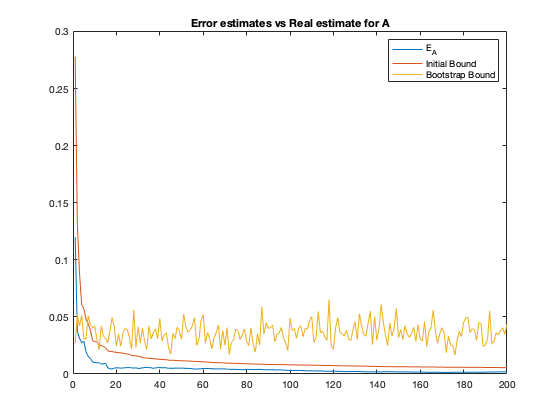
\includegraphics[width=0.9\textwidth]{E_A_results.png}
		\caption{\small Estimates for A. Includes actual error and the data-dependent bounds, as well as the bootstrap error estimates}
		\label{fig:e_a}
	\end{subfigure}%
	\begin{subfigure}{0.5\textwidth}
		\centering
		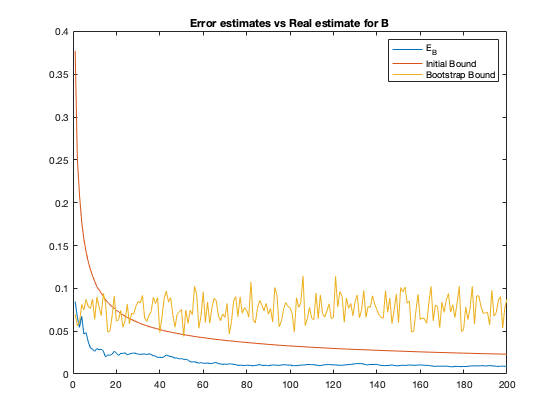
\includegraphics[width=0.9\textwidth]{E_B_results.png}
		\caption{\small Estimates for B. Includes actual error and the data-dependent bounds, as well as the bootstrap error estimates}
		\label{fig:e_b}
	\end{subfigure}
	\caption{Results of numerical example.}
\end{figure}


%\begin{figure}[tb]
%	\centering
%	
%	
%\end{figure}
%
%\begin{figure}[tb]
%	\centering
%	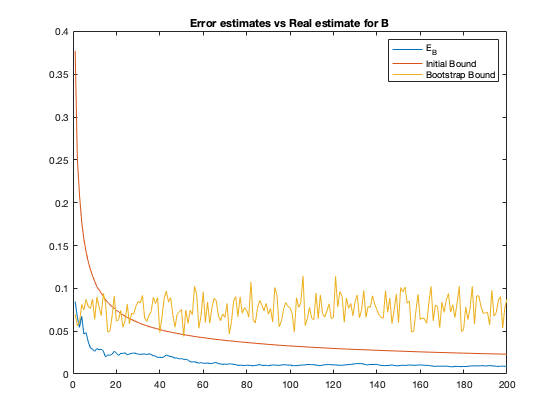
\includegraphics[width=0.3\textwidth]{E_B_results.png}
%	\caption{\small Estimates for B. Includes actual error and the data-dependent bounds, as well as the bootstrap error estimates}
%	\label{fig:e_b}
%\end{figure}

As can be seen from the figure, the data-dependent bounds estimate the overall error across the number of rollouts and improves as the number of rollouts increases.
The bootstrap bound \emph{also shows improvement} (Actually did not work).
\bibliographystyle{IEEEtran}
\bibliography{lec4_bib}

The (very naive and inefficient) code used to derive the results are shown here:
\\ The code for this problem is as follows:
\lstinputlisting{bootstrap_sysID.m}


 \end{document}






